% backward-facing-step.tex
%
\newpage
\section{Backward facing step}
%
The third validation test case is that of a Mach 2.0 flow over a
two-dimensional backward-facing step. Experimental data from Eklund et. al. \cite{Eklund1995}
and McDaniel et. al. \cite{McDaniel1991} are  used for this exercise.

%------------------------------------------------------------------
\subsection{Details of flow problem}
%\label{}
%
The experimental setup used by Eklund et. al. is shown 
schematically in Figure~\ref{backward-facing-step-exp-setup-fig}.
%
\begin{figure}[htbp]
\begin{center}
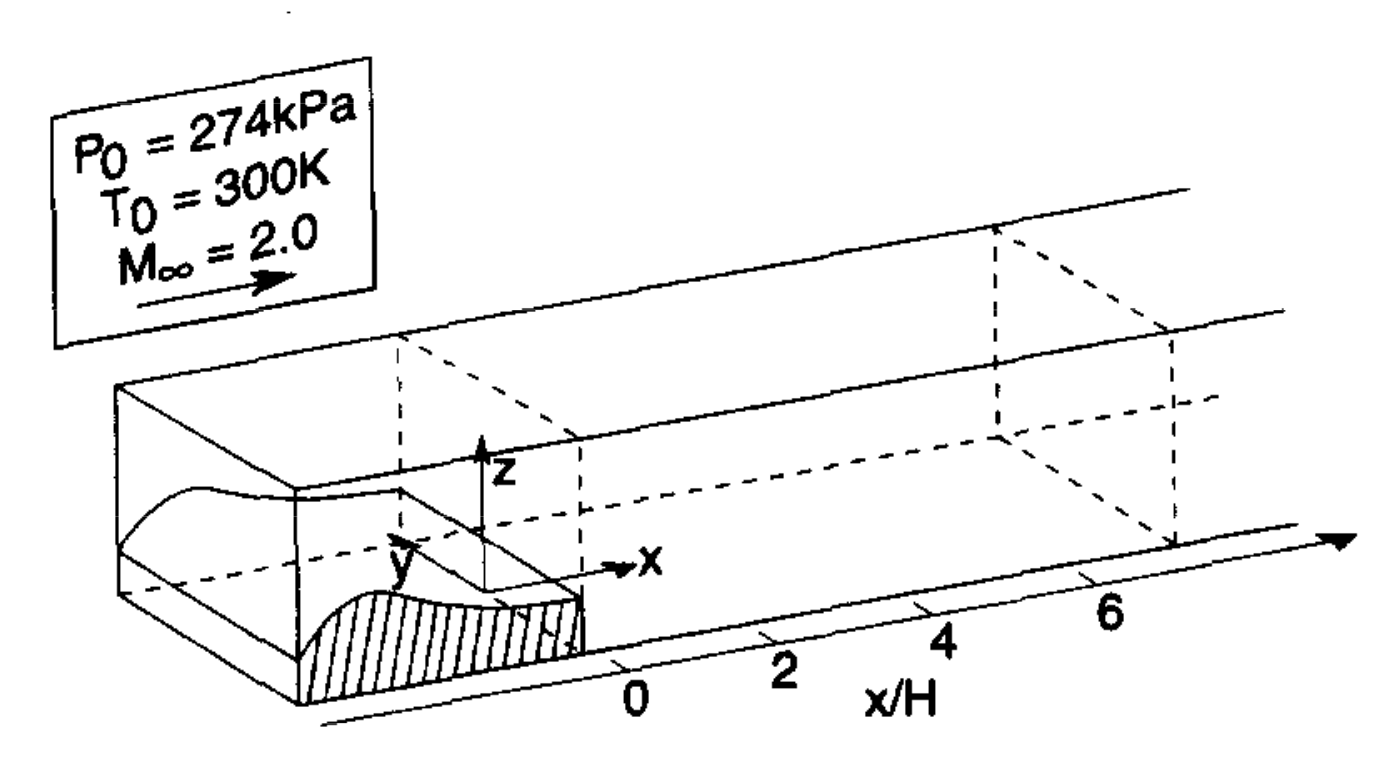
\includegraphics[width=12cm]{./chap4-backward-facing-step/figs/experimental-setup.png}
\end{center}
\caption{Schematic diagram of the experimental setup for the backward
         facing step test case (Reprinted from Eklund et. al. \cite{Eklund1995})}
\label{backward-facing-step-exp-setup-fig}
\end{figure}
%
A two-dimensional Laval nozzle designed to produce a Mach 2 exit flow was 
connected to the backward-facing step via a straight wall. This wall was
slightly angled at 0.5$^{\circ}$ to accommodate boundary layer growth. 
Table~\ref{backward-facing-step-test-section-dims} shows the 
dimensions of the test section in terms of the step height, $H$. The 
nominal inflow conditions of the test section are given in
Table~\ref{backward-facing-step-inflow-conditions}. The inflow boundary 
layer had a thickness of approximately 1.6 mm, and was verified to be 
fully developed and turbulent at one step height distance upstream of 
the step \cite{McDaniel1991}. 
%
\begin{table}[h]
  \caption{Test section geometry}
  \label{backward-facing-step-test-section-dims}
  \begin{center}
    \begin{tabular}{cc}
      \hline\hline
      Feature & Dimension \\
      \hline
      Step height         & $H$=3.175 mm \\
      Test section height & 6.71$H$  \\
      Test section width  & 9.6$H$   \\
      Step location       & $x/H$=0.0 \\
      \hline \hline
    \end{tabular}
  \end{center}
\end{table}
%
\begin{table}[h]
  \caption{Test section nominal inflow conditions}
  \label{backward-facing-step-inflow-conditions}
  \begin{center}
    \begin{tabular}{ccc}
      \hline\hline
      Parameter & & Freestream conditions \\
      \hline
      Stagnation pressure    & $P_0$      & 274 kPa \\     
      Stagnation temperature & $T_0$      & 300 K   \\   
      Mach number            & $T_0$      & 2.0     \\
      Static pressure        & $P_\infty$ & 35 kPa  \\  
      Static temperature     & $T_\infty$ & 167 K   \\
      $u$-velocity           & $u_\infty$ & 518 m/s \\
      \hline \hline
    \end{tabular}
  \end{center}
\end{table}
Three types of measurement techniques were used for flowfield measurements
in these experiments - pointwise Laser-Induced Iodine Fluorescence (LIIF),
Planar Laser-Induced Iodine Fluorescence (PLIIF) \cite{McDaniel1991, McDaniel1993} 
, and Laser Doppler Anemometry (LDA). LIIF 
techniques are non-intrusive optical techniques that infer flowfield
properties from signals resulting from the laser-induced fluorescence of
iodine molecules seeded into the flow. The pointwise LIIF technique was 
used to produce pointwise measurements of pressure, temperature and velocity
in the test section. In contrast to the pointwise LIIF technique, the PLIIF 
technique was used to produce planar measurements of pressure, temperature and 
velocity. Laser Doppler Anemometry, a well-established technique for pointwise
velocity measurement, was used in these experiments to measure the mean velocities 
and their fluctuations. Since the LIIF and PLIIF techniques provided only 
time-averaged data, the LDA data was an important addition to the data set in 
providing information about the turbulence intensity in the flow field.

Eilmer3 results are compared to profiles of pressure, temperature, and 
$u$-velocity obtained via the pointwise LIIF technique at seven positions along the 
centerline of the test section that correspond to $x/H$ locations of -1.0, -0.1, 1.7, 
3.0, 3.9, 6.7 and 10.8. The comparisons at $x/H$ = -1.0 are made to confirm that
Eilmer3 simulations of the inflow to the step are correct. Contour plots of pressure 
and temperature obtained numerically are also compared with planar measurements 
obtained via the PLIIF technique. 

The uncertainties of the various experimental techniques used in the 
acquisition of the data sets are listed in Table~\ref{backward-facing-step-uncertainties}. 
The uncertainties are quoted as a percentage of the freestream conditions in 
Table~\ref{backward-facing-step-inflow-conditions}. The actual 
uncertainties in the PLIIF images may be larger than those listed in 
Table~\ref{backward-facing-step-uncertainties} in certain regions of the image, as will be
discussed in Section~\ref{backward-facing-step-results}. Absolute spatial positioning error 
for all measurement techniques was less than $\pm$50 $\mu$m, or $\pm$1.6\% of the step 
height, $H$. 

%The spatial positioning was inherently more precise in the PLIIF 
%techniques than in the pointwise techniques. The spatial measurement volume 
%was approximately 0.001 mm$^3$ for the LIIF and PLIIF techniques and 
%approximately 0.01 mm$^3$ for the LDA technique. \\

\begin{table}
  \caption{Experimental uncertainties (from \cite{McDaniel1991}) }
  \label{backward-facing-step-uncertainties}
  \begin{center}
    \begin{tabular}{ccc}
      \hline\hline
      Technique & Parameter & Uncertainty \\
      \hline
      LIIF  & $P$ & $\pm$4\%\\
            & $T$ & $\pm$2\%\\
            & $u$ & $\pm$5\%\\
      PLIIF & $P$ & $\pm$6\%\\
            & $T$ & $\pm$5\%\\
            & $u$ & $\pm$2\%\\
      LDA   & $u$, $w$   & $\pm$2\%\\
            & $u'$, $w'$ & $\pm$2\%\\
      \hline \hline
    \end{tabular}
  \end{center}
\end{table}

%-----------------------------------------------------------------
\subsection{Details of computational approach}
%\label{}
%
The computational mesh used is shown in Figure~\ref{backward-facing-step-computational-mesh}.
Note that the Laval nozzle present in the experiments was not modelled. In place of this,
a two-dimensional duct with a 0.5$^{\circ}$ slope to accommodate boundary layer growth
was used. The overall length of the duct was adjusted until the simulated boundary
layer profiles match the experimentally measured profiles at $x/H$ = -1.0. The
turbulence intensity and turbulent-to-laminar viscosity ratio were also adjusted
so that the turbulence intensity matched that measured at $x/H$ = -1.0 using
the LDA technique. The turbulence intensity and turbulent-to-laminar viscosity ratio used
for these simulations are 1\% and 100 respectively. Since the turbulence intensity and 
turbulent-to-laminar viscosity ratio were also fixed, sensitivity studies of the results 
to these freestream turbulence properties were not conducted.

The inflow parameters were specified as per Table~\ref{backward-facing-step-inflow-conditions}. 
Air with an ideal gas assumption, a constant specific heats ratio of 1.4 and a 
gas constant of 287.1 J/kg.K was used as the test gas for the simulations.
\begin{figure}[h]
 \begin{center}
  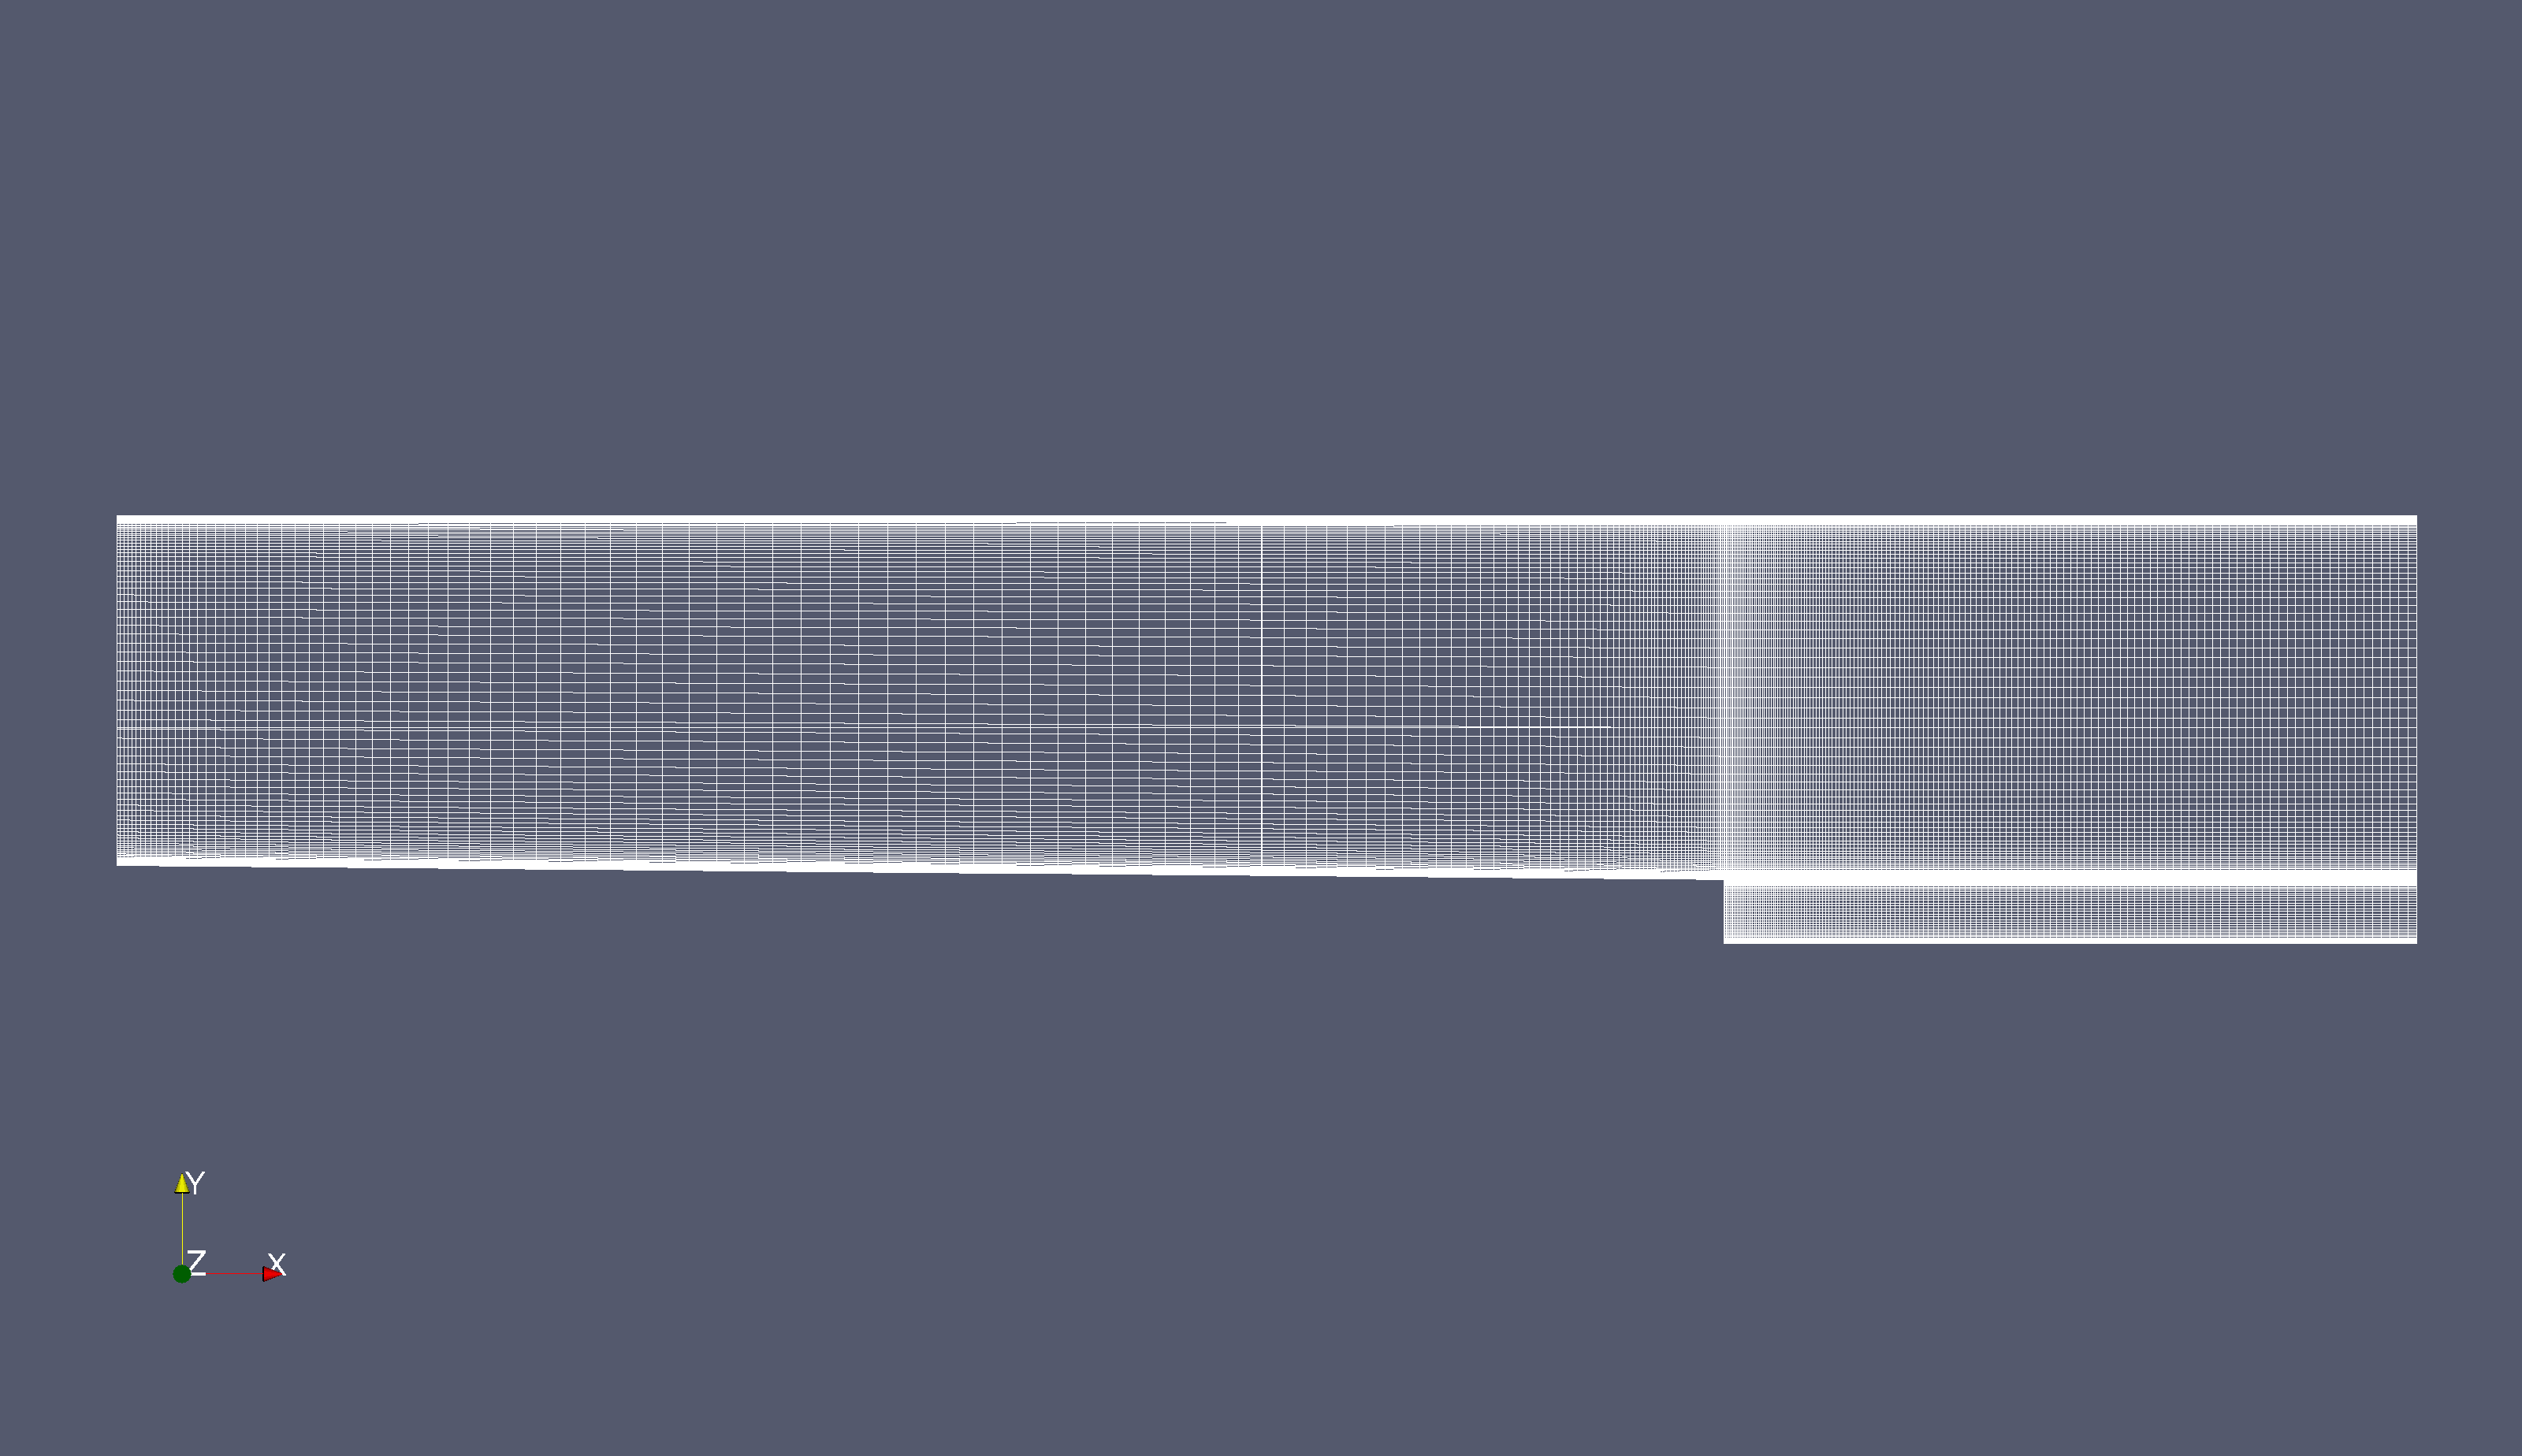
\includegraphics[width=10cm]{./chap4-backward-facing-step/figs/grid.png}
 \end{center}
 \caption{Computational mesh}
 \label{backward-facing-step-computational-mesh}
\end{figure}
Three sets of grids were used for this test case - a fine grid (40080 cells), 
a medium grid (10020 cells), and a coarse grid (2685 cells). The $y^+$ (or $z^+$ 
for the coordinate system used in this section) for the grids were lesser than 1.0, 
except in the first few wall cells from the leading edge where the boundary layer 
was establishing. It was also ensured that there were at least 15 cells within the
boundary layer for most parts of the computational domain.

%-----------------------------------------------------------------
\subsection{Grid convergence}
%\label{}
%
Figures~\ref{backward-facing-step-xH--01} - \ref{backward-facing-step-xH-108}
show that sufficiently grid-resolved results can be obtained from Eilmer3 simulations
using the fine grid.

%------------------------------------------------------------------
\subsection{Results \& discussions}
\label{backward-facing-step-results}
%
Comparisons between numerical predictions and experimental data are firstly
made for the inflow upstream of the step at $x/H$ = -1.0. Comparisons will then
be made with the PLIIF measurements and with the pointwise LIIF measurements.

A comparison of the numerical and experimental profiles at one step height
($x/H$ = -1.0) upstream of the step is shown in Figure~\ref{backward-facing-step-xH--10}.
Three minor discrepancies can be observed. Firstly, the numerical simulations did not
predict as much fluctuations in the pressure level as in the experimental data.
Considering that the actual 2D Laval nozzle was not being modelled due to the 
unavailability of nozzle geometrical information, and that the average pressure
levels matches the experimental data, this discrepancy is deemed acceptable. Secondly,
the numerical simulations seem to overpredict the temperature in the region
near the walls. For the PLIIF technique employed, the fluorescence signal 
decreases with increasing temperature. For this reason, an increment in the measured 
signal owing to background scattering near tunnel walls can substantially lower measured
temperatures \cite{Eklund1995}. These low temperature measurements in the region near the wall
can be consistently seen in later comparisons made with PLIIF and LIIF data. Thirdly,
despite matching the turbulence intensity levels in the freestream of the flow,
the turbulence intensity near the walls are underpredicted. The experimental 
turbulence intensity is the root-mean-square value of $u$-velocity fluctuations
normalised by freestream $u$-velocity, $\sqrt{u^{'2}}/u_{\infty}$, while 
the numerical turbulence intensity is the square-root of two-thirds of the turbulence 
kinetic energy normalised by freestream $u$-velocity, $\sqrt{\frac{2}{3}k}/u_{\infty}$. 
The assumption that $\sqrt{u^{'2}}$ is equal to $\sqrt{\frac{2}{3}k}$ is only valid if
the turbulence is isotropic. However, in most turbulent shear flows, where turbulence
is anisotropic, $\sqrt{u^{'2}}$ is slightly larger than $\sqrt{\frac{2}{3}k}$ \cite{Hinze1975}.
As such. the comparison between experimental and numerical turbulence intensities
in Figure~\ref{backward-facing-step-xH--10} should only be treated as an
approximate one. Apart from these discrepancies, the overall agreement between the
numerical and experimental profiles upstream of the step is excellent. This allows
a more confident assessment of the numerical predictions of the flow past the step
to be made.
%
\begin{figure}[h]
 \begin{center}
  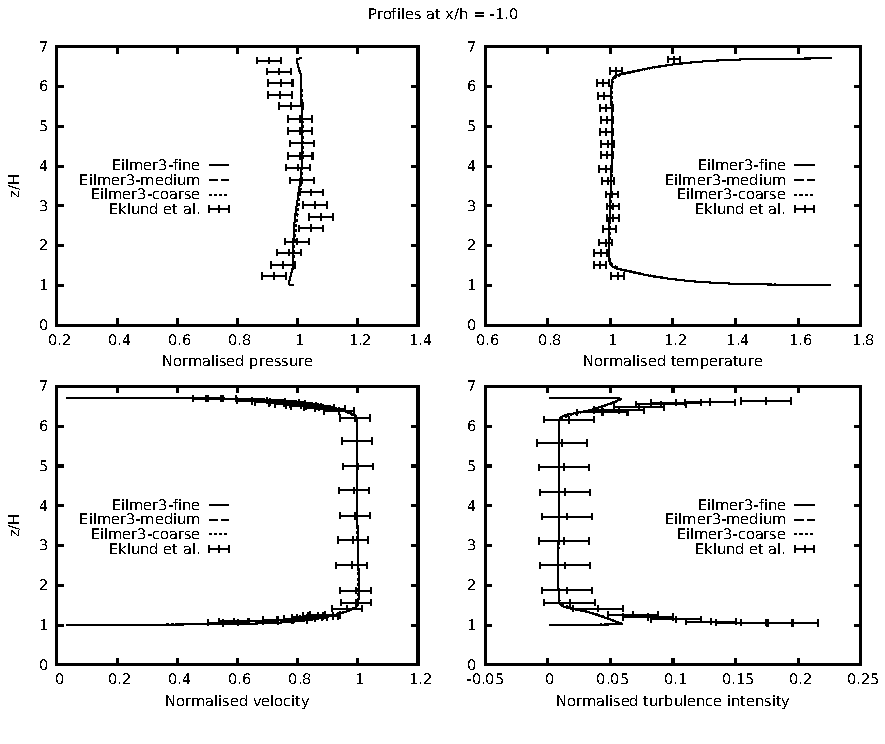
\includegraphics[width=15cm]{./chap4-backward-facing-step/figs/xh_-10.pdf}
 \end{center}
 \caption{Boundary layer profiles at $x/H$ = -1.0}
 \label{backward-facing-step-xH--10}
\end{figure}
%

Eilmer3 predictions of flow past the step are shown together with experimental
PLIIF measurements in Figures~\ref{figure-backward-step-pressure-contours} and 
\ref{figure-backward-step-temperature-contours}. 
Figure~\ref{figure-backward-step-pressure-contours} shows that the
%
\begin{figure}[h]
 \centering
 \subfigure[]{
   \label{figure-backward-step-pressure-contours-a}
   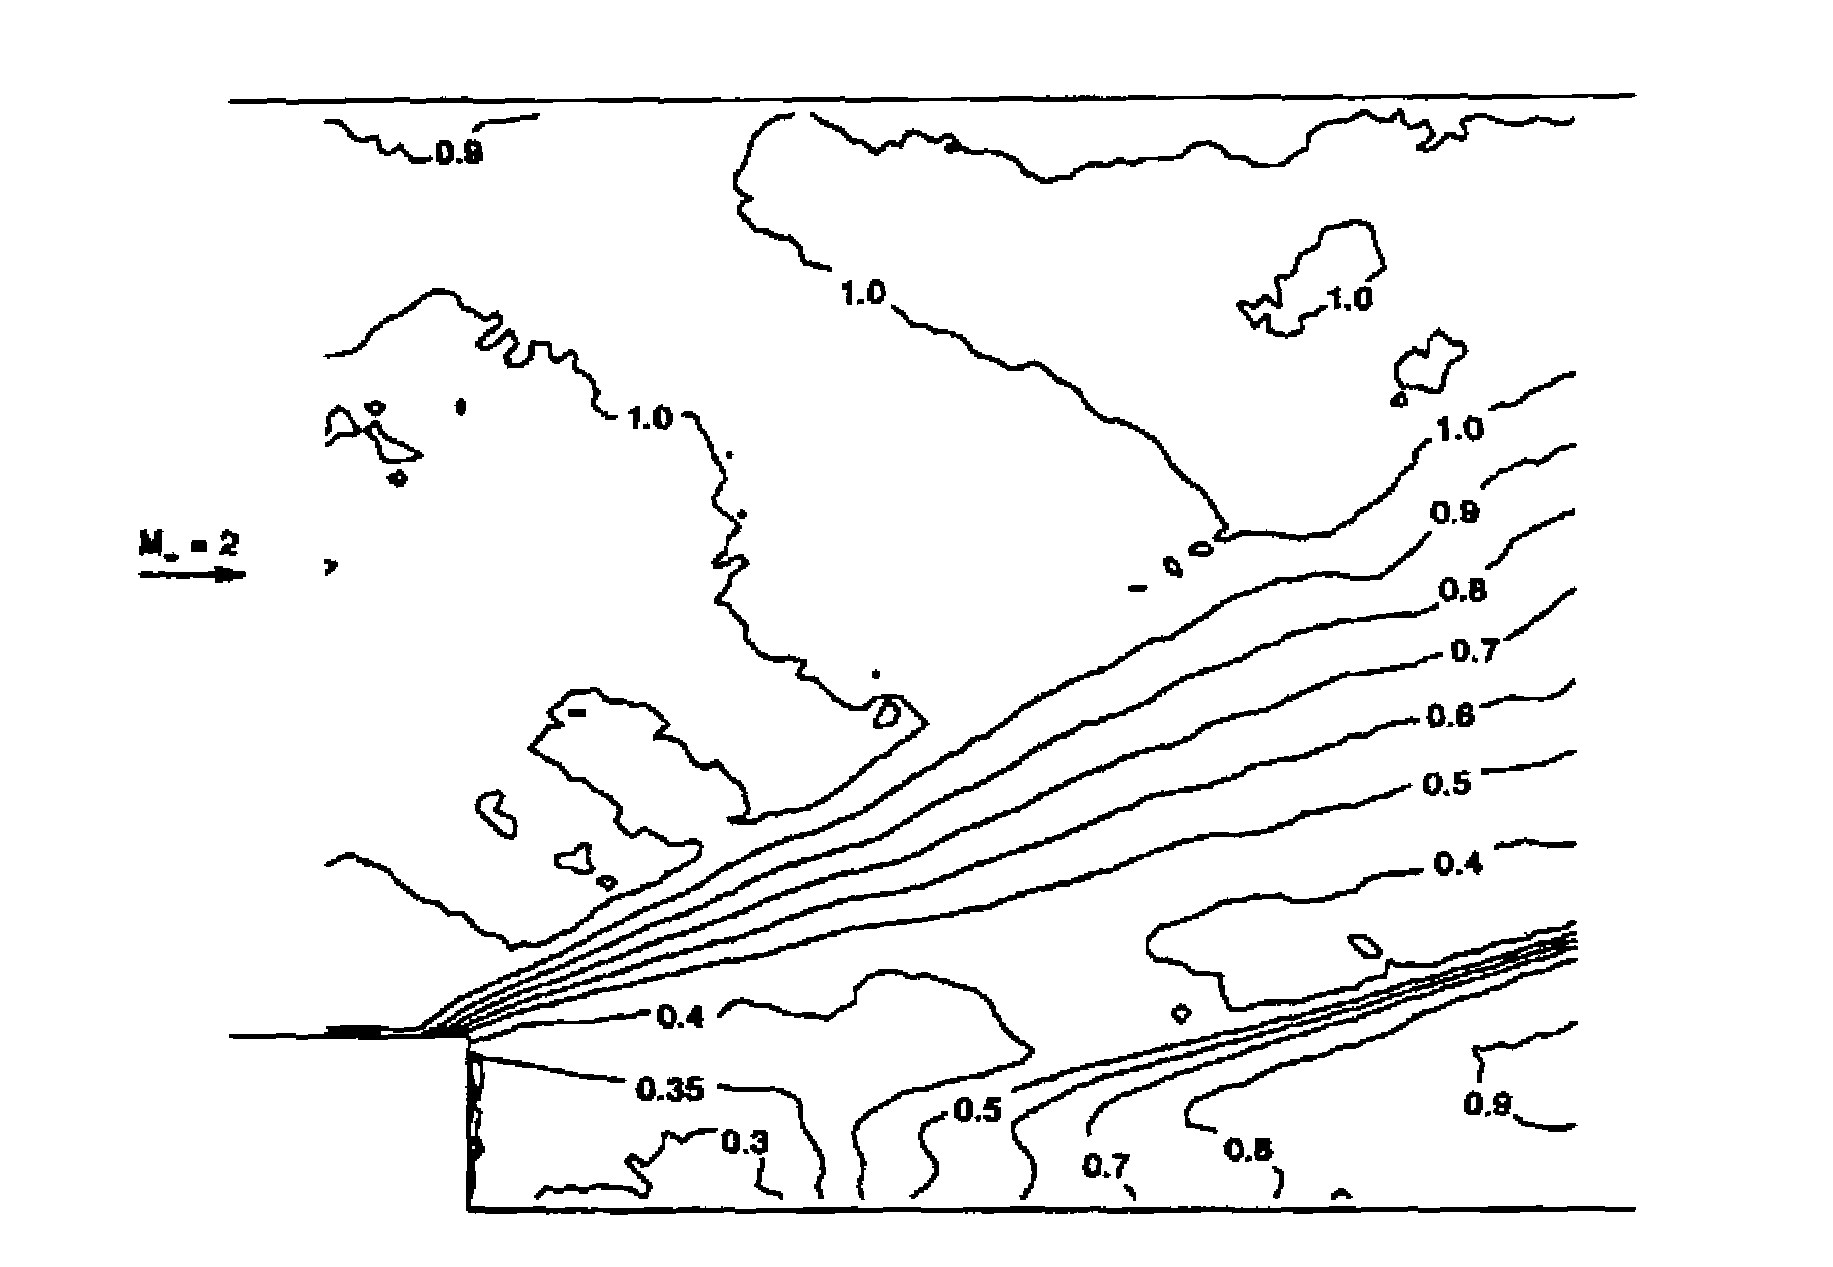
\includegraphics[width=14cm]{./chap4-backward-facing-step/figs/pressure_contours_exp.pdf}
 }
 \subfigure[]{
   \label{figure-backward-step-pressure-contours-b}
   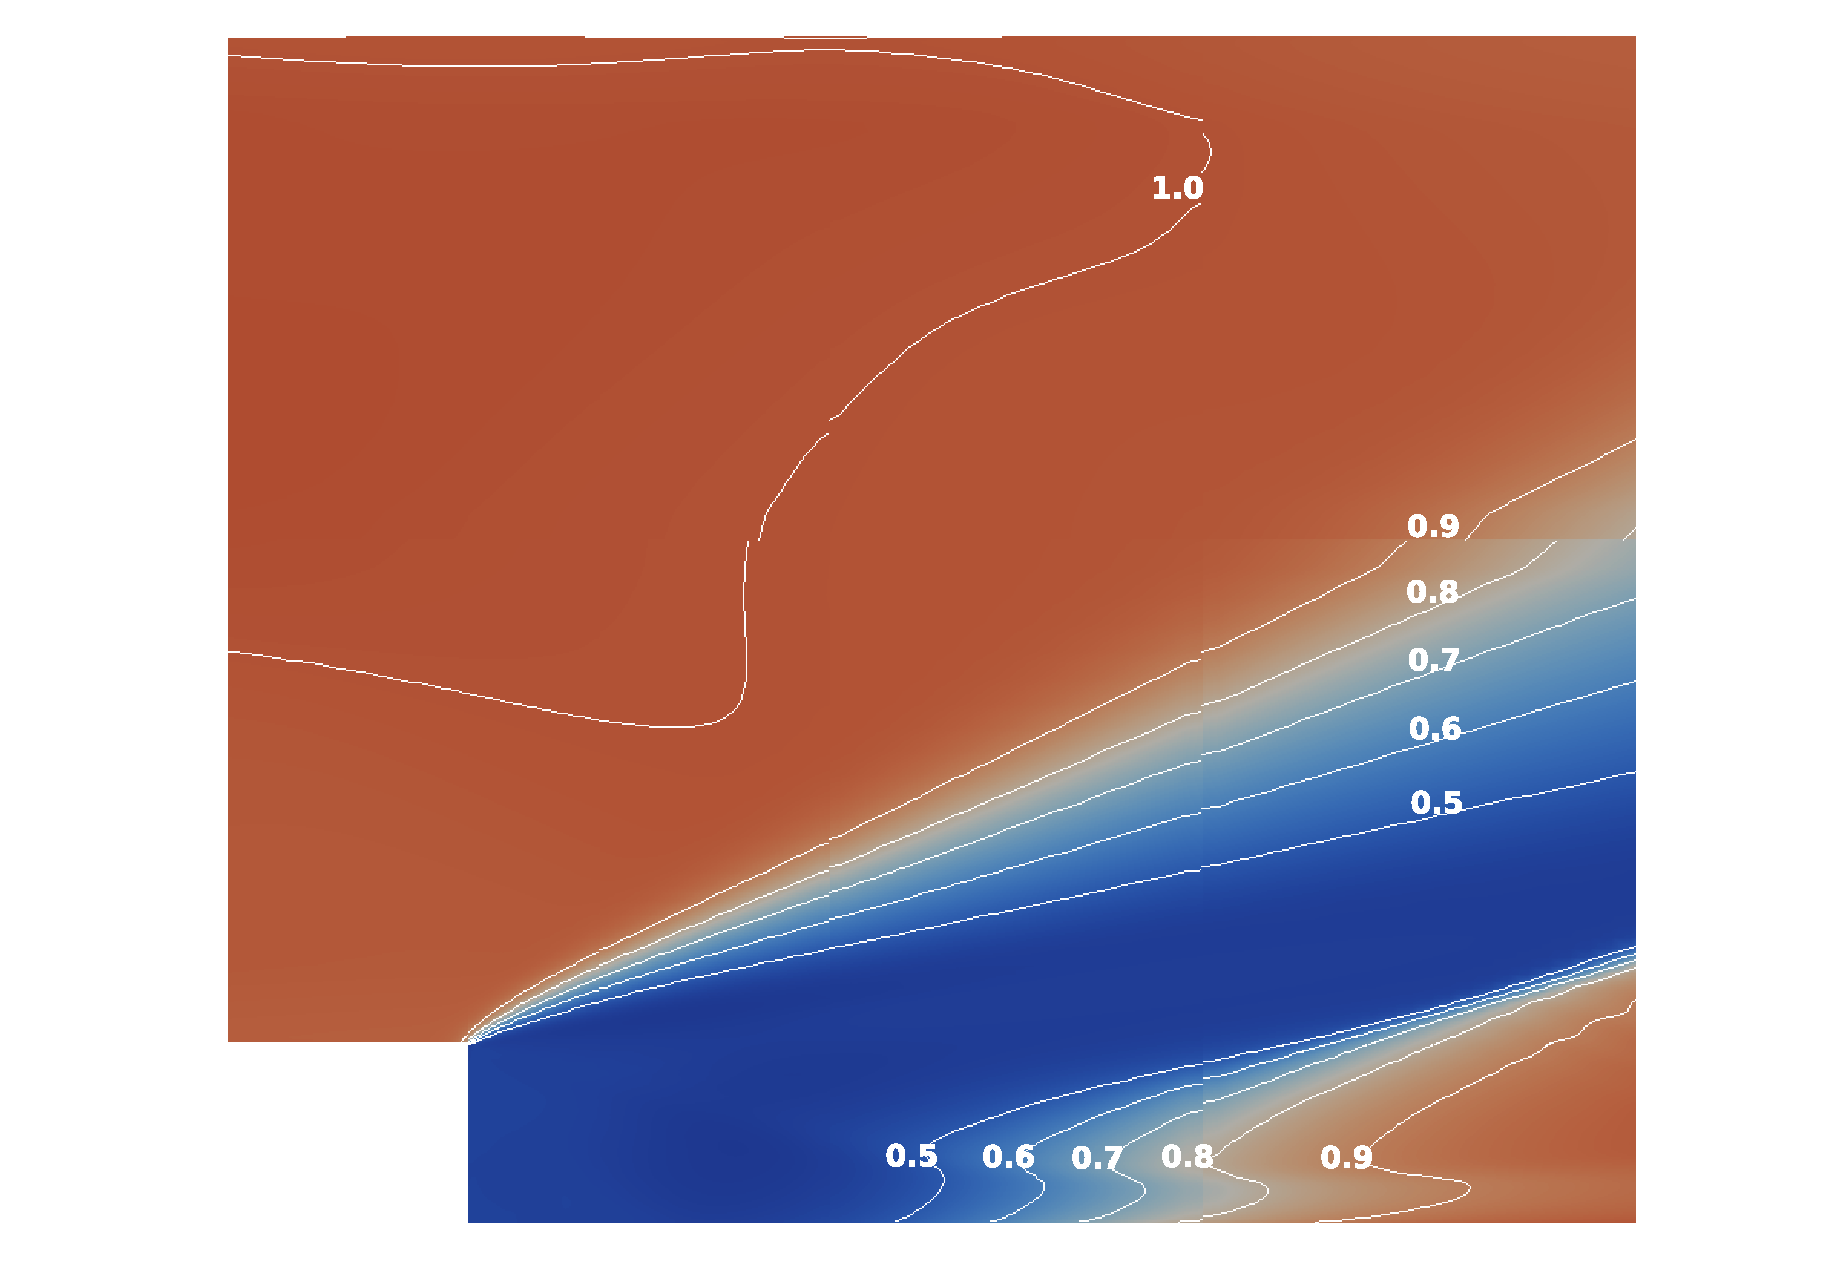
\includegraphics[width=14cm]{./chap4-backward-facing-step/figs/pressure_contours_num.pdf}
 }
 \caption{Comparison between (a) experimentally measured and (b)
          numerically simulated pressure contours}
 \label{figure-backward-step-pressure-contours}
\end{figure}
%
\begin{figure}[h]
 \centering
 \subfigure[]{
   \label{figure-backward-step-temperature-contours-a}
   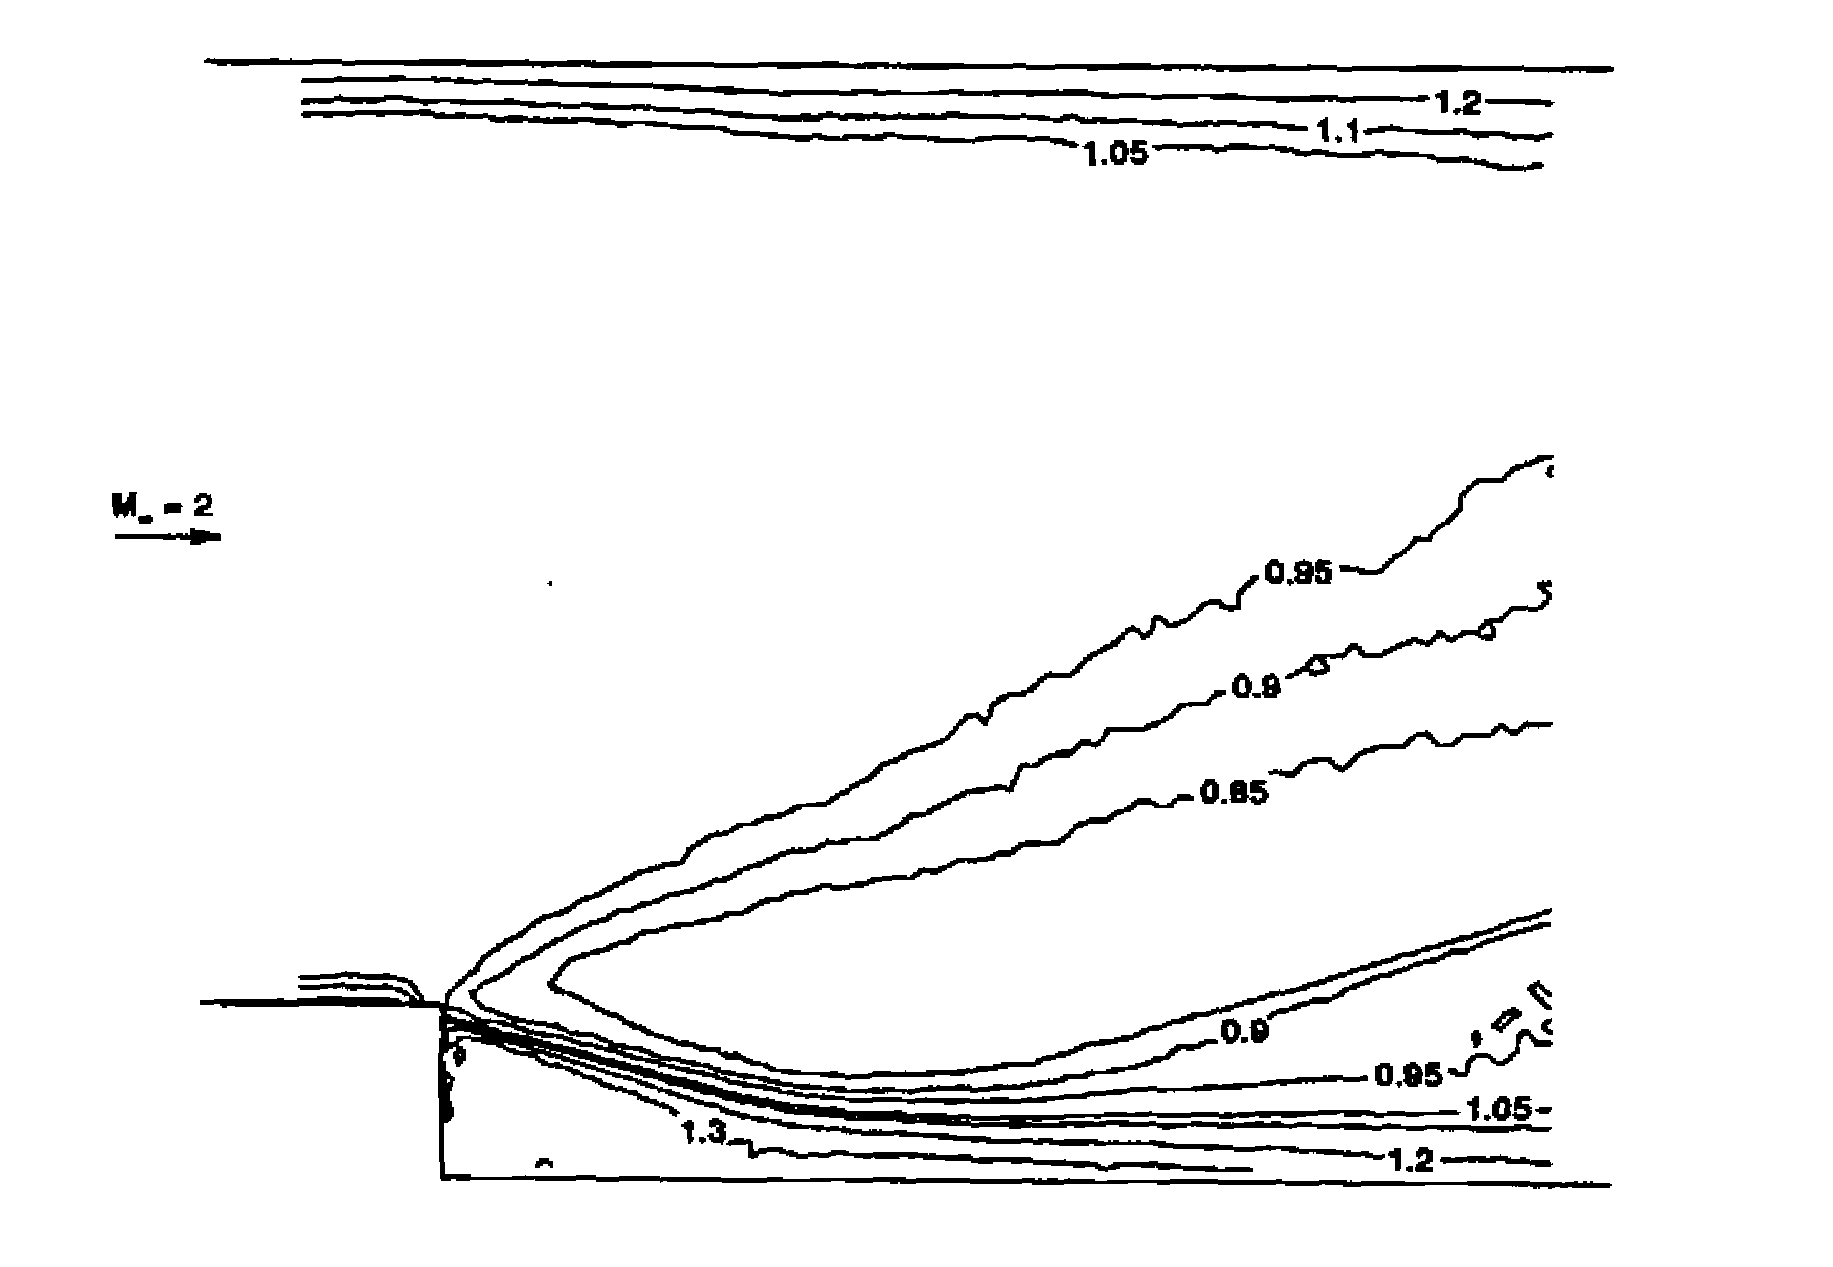
\includegraphics[width=14cm]{./chap4-backward-facing-step/figs/temperature_contours_exp.pdf}
 }
 \subfigure[]{
   \label{figure-backward-step-temperature-contours-b}
   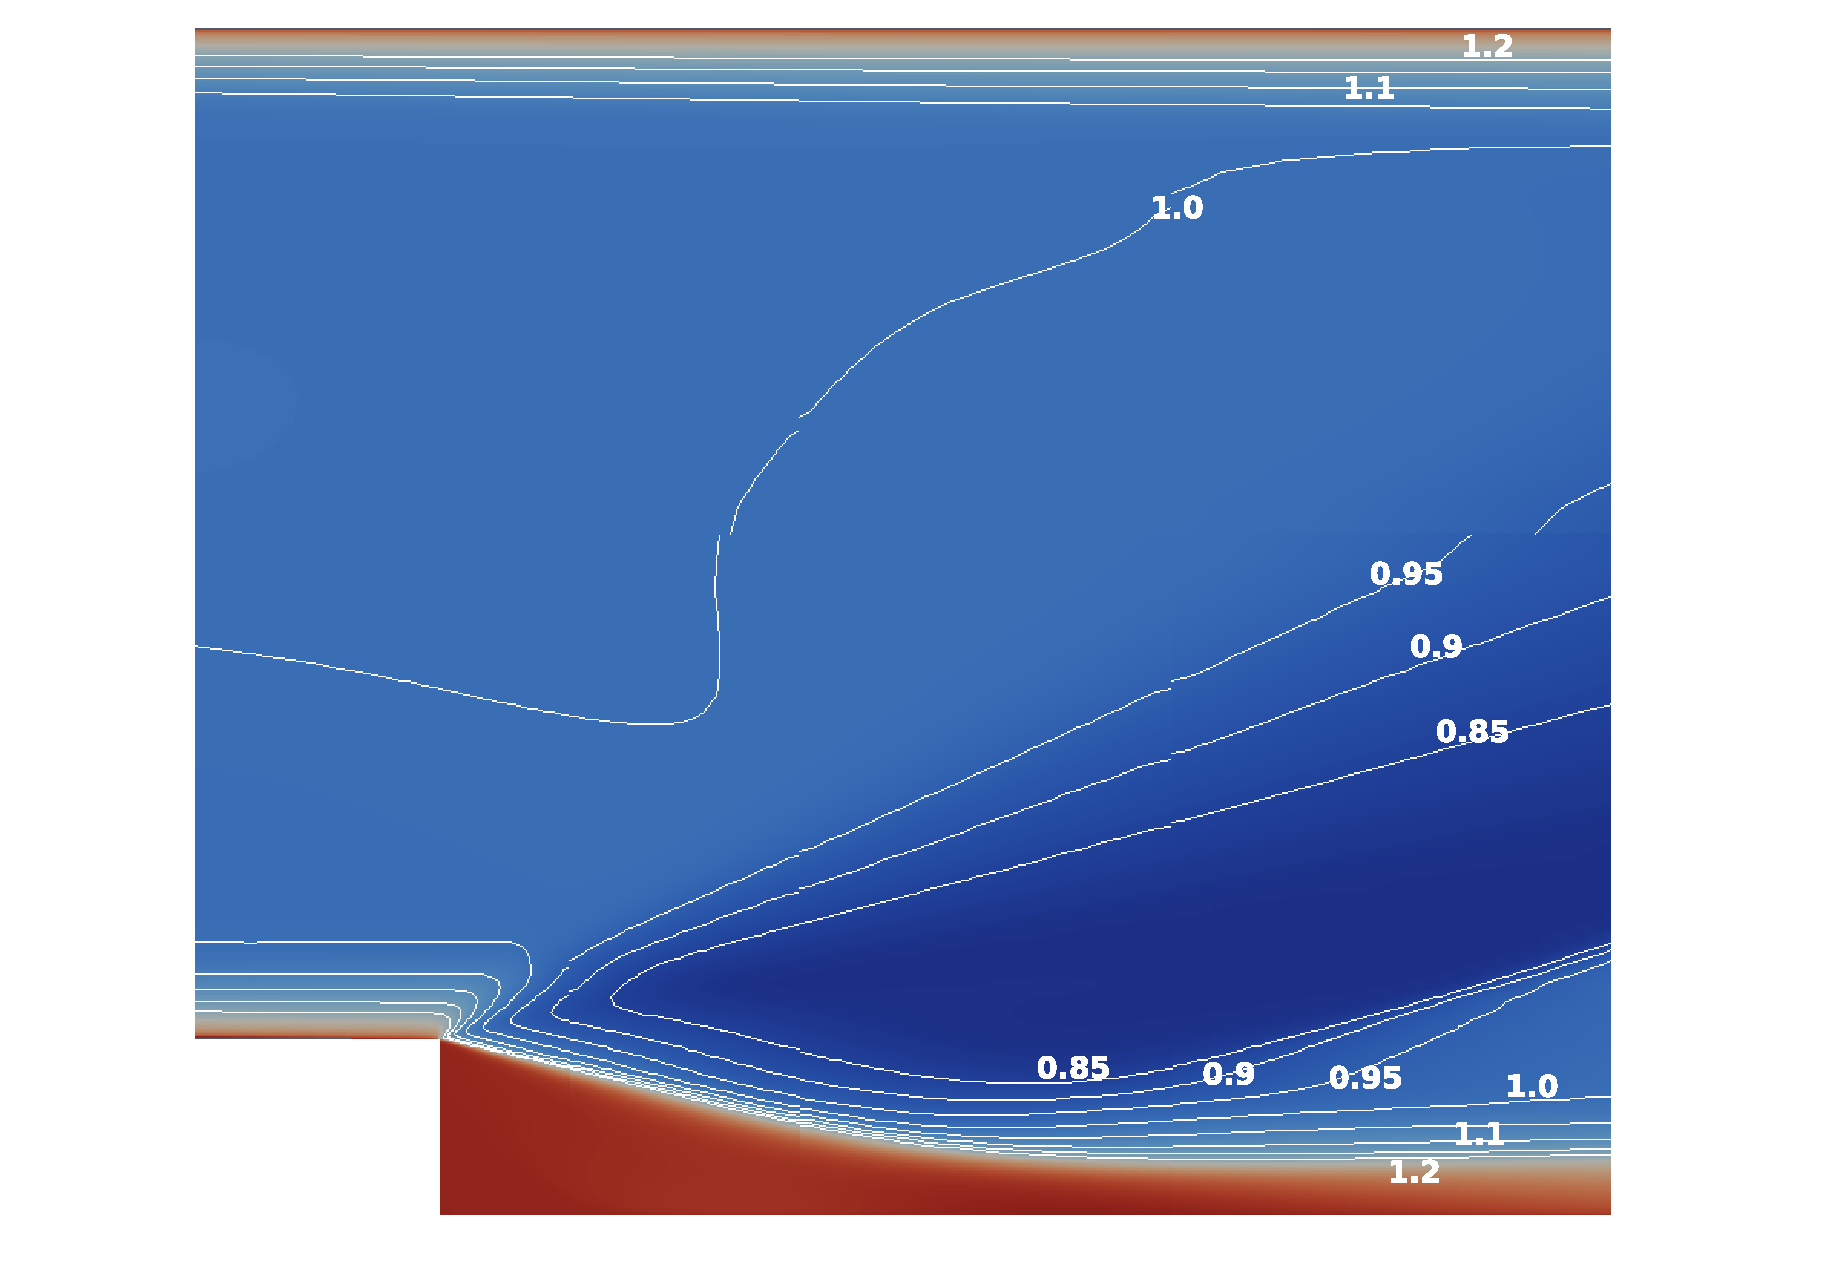
\includegraphics[width=14cm]{./chap4-backward-facing-step/figs/temperature_contours_num.pdf}
 }
 \caption{Comparison between (a) experimentally measured and (b)
          numerically simulated temperature contours}
 \label{figure-backward-step-temperature-contours}
\end{figure}
%
degree of expansion and reattachment shock angle are well predicted. Only 
two minor differences can be seen. Firstly, the expansion fan is predicted 
to centre around the step and does not extend as far upstream as measured 
in the experiments. Eklund et. al. \cite{Eklund1995} explained
that the occurence of the expansion fan further upstream of the step was
attributed to the suction effect from the low pressure region in the base region
of the step. This phenomena is not predicted by the Eilmer3 simulations probably because
the slight curvature that was present at the corner of the step was not modelled. 
This curvature was mentioned in the paper of Eklund et. al. \cite{Eklund1995}, but no geometrical
information was provided. The second difference is that the recompression is predicted 
to begin further upstream than in the experimental PLIIF measurements. This is 
despite the recompression shock angle being predicted correctly. This results in 
higher pressure levels in the vicinity.
Figure~\ref{figure-backward-step-temperature-contours} shows good agreement between 
the predicted and measured temperatures everywhere in the flowfield other than in 
the region near the walls. As discussed earlier, Eilmer3 predicts higher temperature 
levels than measured. This mismatch is due to the erroneous near-wall PLIIF measurement 
of temperatures brought about by background scattering.

Comparisons between the predicted and measured profiles of pressure, temperature
and $u$-velocity at several axial locations are shown in Figures~\ref{backward-facing-step-xH--01} - \ref{backward-facing-step-xH-108}.
The good agreement observed earlier between Eilmer3 predictions and PLIIF measurements
is also seen when comparing the predictions with pointwise LIIF measurements.
The differences observed earlier can also be seen in this comparison. 
The discrepancy in the prediction of the origin of the expansion fan can be seen in
the pressure profiles at $x/H$ = -0.1. The start of recompression shock is however 
different from the PLIIF comparisons, with it being predicted to occur downstream, 
as shown at $x/H$ = 3.9. The systematically low temperatures measured in the vicinity 
of the wall is seen again at every axial location. In summary, the overall agreement of 
Eilmer3 predictions with the experimental data is excellent.
%
\begin{figure}[h]
 \begin{center}
  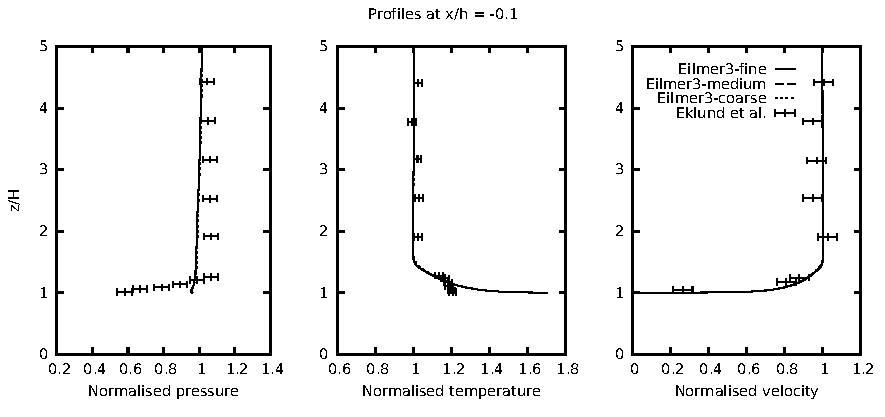
\includegraphics[width=13.8cm]{./chap4-backward-facing-step/figs/xh_-01.pdf}
 \end{center}
 \caption{Boundary layer profiles at $x/H$ = -0.1}
 \label{backward-facing-step-xH--01}
\end{figure}
%
\begin{figure}[h]
 \begin{center}
  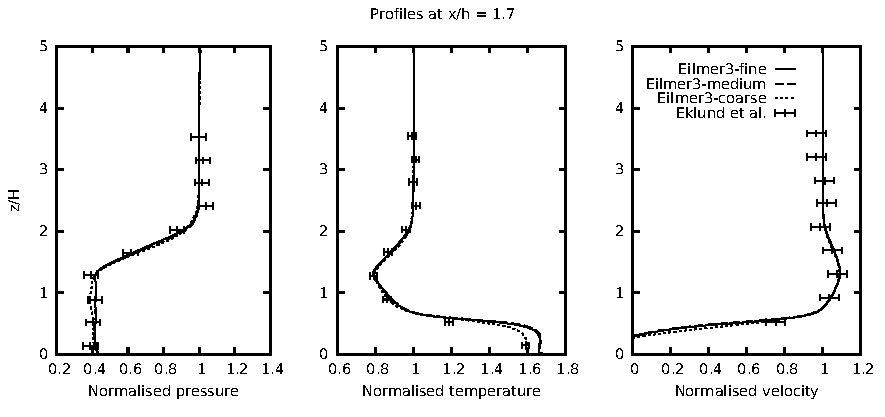
\includegraphics[width=13.8cm]{./chap4-backward-facing-step/figs/xh_17.pdf}
 \end{center}
 \caption{Boundary layer profiles at $x/H$ = 1.7}
 \label{backward-facing-step-xH-17}
\end{figure}
%
\begin{figure}[h]
 \begin{center}
  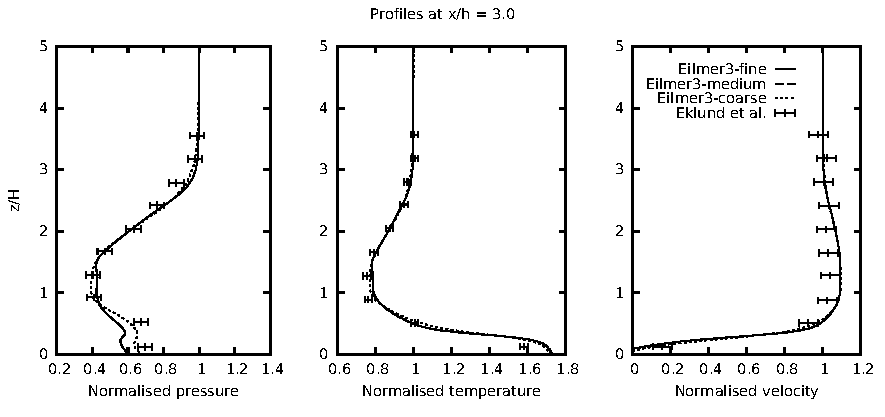
\includegraphics[width=13.8cm]{./chap4-backward-facing-step/figs/xh_30.pdf}
 \end{center}
 \caption{Boundary layer profiles at $x/H$ = 3.0}
 \label{backward-facing-step-xH-30}
\end{figure}
%
\begin{figure}[h]
 \begin{center}
  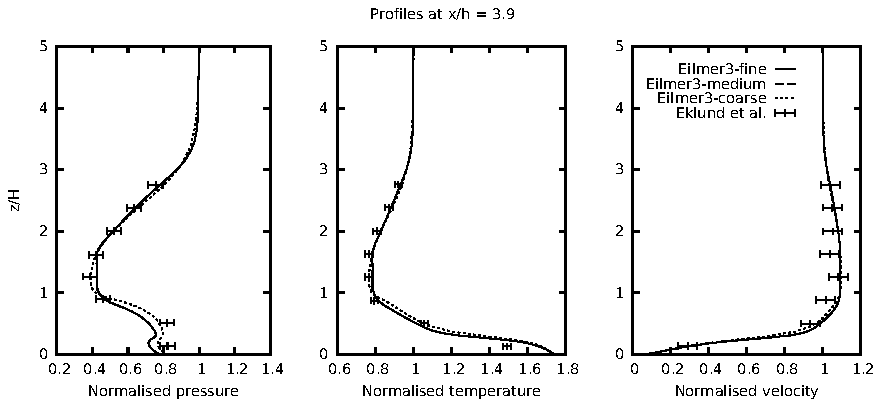
\includegraphics[width=13.8cm]{./chap4-backward-facing-step/figs/xh_39.pdf}
 \end{center}
 \caption{Boundary layer profiles at $x/H$ = 3.9}
 \label{backward-facing-step-xH-39}
\end{figure}
%
\begin{figure}[h]
 \begin{center}
  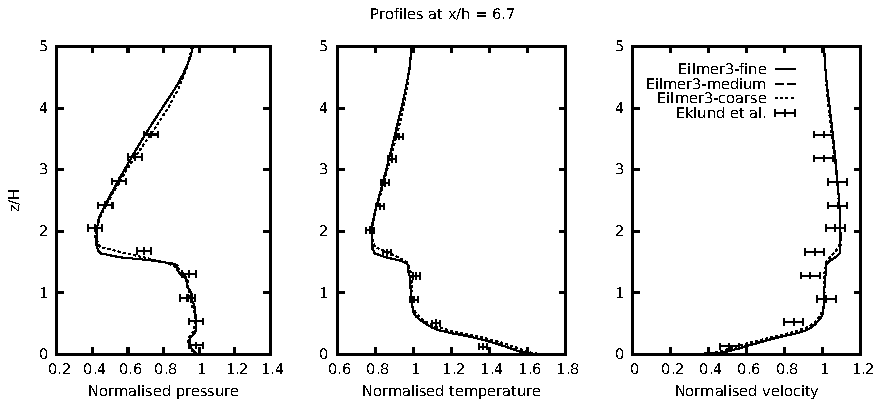
\includegraphics[width=13.8cm]{./chap4-backward-facing-step/figs/xh_67.pdf}
 \end{center}
 \caption{Boundary layer profiles at $x/H$ = 6.7}
 \label{backward-facing-step-xH-67}
\end{figure}
%
\begin{figure}[h]
 \begin{center}
  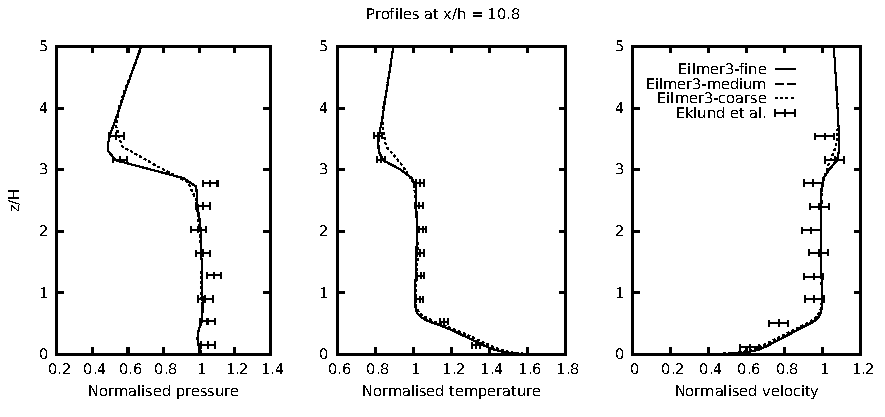
\includegraphics[width=13.8cm]{./chap4-backward-facing-step/figs/xh_108.pdf}
 \end{center}
 \caption{Boundary layer profiles at $x/H$ = 10.8}
 \label{backward-facing-step-xH-108}
\end{figure}
%

%------------------------------------------------------------------


